\chapter{Finite State Machines}
\label{chapter:Finite State Machines}
\graphicspath{ {./chapter07/Fig} }

In Chapter 5 the exploration began with sequential circuits, circuits
whose output is a function of the input and current state, and by examining
the basic memory elements. Now, utilization of these basic
memory elements to build general sequential circuit is considered.

The sequential design process starts the same as the combination design
process, with a word statement.  From this word statement, a state diagram is created.
The logic to control the transitions between the
states is derived directly from
the state diagram.  In cases where the finite state machine (FSM) controls a
complex system, it may be necessary to build a control word table to
determine the output equations.  Otherwise, the output equations are derived
directly from the state diagram.  In order to make this discussion more
concrete, all the FSMs to be designed in this chapter have the
structure shown in Figure~\ref{fig:sequentialFSMGenFSM}.

\begin{figure}[ht]
    \center{\scalebox{1.0}{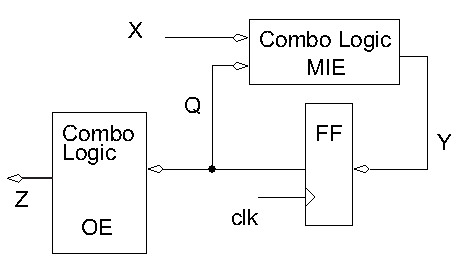
\includegraphics{GenFSM}}}
    \caption{The standard structure of a FSM for the current chapter.}
    \label{fig:sequentialFSMGenFSM}
\end{figure}
\label{page:GenFSM}

Each of the signals $X,Y,Q,Z$ is a vector, consisting of zero or more bits.
The $X$ signal is the input to the FSM from the system being controlled.
The $Z$ signal is the output from the FSM to the system being controlled.
The combinational logic circuit generating $Z$ is called the \textit{ output
equations} (OE).  The state of the FSM is carried on the $Q$
lines.  Each bit of $Q$ is the output of a D flip flop. Thus, if $Q$ is
six bits wide, then the FSM has six D flip flops.  The $Y$ signals are
called the
memory inputs; they are the data inputs to the D flip flops.  The combinational
logic circuit generating the $Y$ signals is called the \textit{ memory input
equations} (MIEs). In order to improve the readability of circuit
diagrams, from now on, the clock signal will not be shown.
With respect to Figure~\ref{fig:sequentialFSMGenFSM}, the design
of a FSM requires three questions be answered: What are the MIEs; what
are the OEs; and how many D flip flops are required?  These questions are
answered by first understanding how to convert a word statement into a state
diagram.

\section{Word Statement to State Diagram}

Since the design of a FSM starts with the conversion of a word statement into
a state diagram, it is imperative to understand what information is captured
in the states of a state diagram.

The states of a FSM can be thought of as the history of previous
inputs, the operating modes of a system, or the steps in a process.

A state can be used to capture the history of previous inputs.  For example,
consider a FSM controlling a vending machine which dispenses
35\textcent sodas.  The
FSM has two bits of inputs, N and D which equal 1 when a nickel or dime is
inserted.  It has one bit of output which equals when to dispense a soda.  The
states in this FSM would represent how much money has been deposited so far.

A state can be used to capture the operating mode of a system.  For example,
the FSM which controls a furnace in a house might have two states;
on or off.

A state can be used to capture which step a process is in.  For example,
consider a FSM which controls the movement of milking cows through a chute
in order to read their ID tags.  The FSM has two inputs, one which detects
if a cow is present in the chute and the other if the ID tag has been
read correctly. The FSM has two outputs, each controlling the position of either
the entrance or exit gates.  The FSM has states such as CowPresent,
WaitToConfirmRead, WaitForCowToLeave, etc..

Regardless of what the states represent, the state diagram must be drawn in the
same standardized way.  Each state name is drawn inside a circle.
One of the states is selected to be the state the FSM starts in when
first powered-up.  This state, referred to as the reset state, is
denoted by putting an asterisk inside its
circle.  The FSM is in exactly one state at a given time.  When the clock edge
arrives, the FSM samples its inputs and transitions to a next state.  Outgoing
arcs from the state are labeled with the input condition which elicits the
corresponding transition.  As mentioned in Chapter 5, the collection of
outgoing arcs from a state should be complete and unequivocal.  Complete means
that every possible combination of the variables used on the outgoing arcs has
been described.  Unequivocal means  no ambiguity in the decision of
the next state exists.

%%----------------State Diagram to Circuit Diagram------------

\section{Design Using Ones Hot Encoding}

In order to transform an abstract state diagram into a real circuit, the
symbolic state names in the state diagram must be given some binary encoding.
When the FSM is in a particular state, $S$, the binary coding for $S$
is present on the outputs of the flip flops; $Q$ in Figure~\ref{fig:sequentialFSMGenFSM}.
Many different ways can be proposed to choose the encoding of states.  The two most
popular are dense and one-hot.

A dense encoding minimizes the number of bits used to encode the
states.  This approach
is a reasonable goal as minimizing the number of bits to encode the states
has the effect of minimizing the number of flip flops in the FSM.  According to
the arguments made on page~\pageref{page:two-to-N}, if a state diagram has $N$
states, then each can be assigned a unique binary code using $log_2(N)$ bits.
For example, if the vending machine state diagram mentioned earlier had eight
states, then its FSM designed using a dense encoding of states requires
three bits.  These three bits could be arranged in eight different ways, each representing
one of the states.  Consequently, its FSM would have three flip flops.

A one-hot encoding assigns one flip flop to each state.  When the FSM is in
state $S$, the flip flop associated with state $S$ outputs 1. Since a FSM can
only be in one state at a time, exactly one flip flop in a one-hot encoded FSM
outputs 1 and all the others output 0.  The name ``one-hot" refers to the
fact that one of the flip flop outputs is ``hot" or at a logic 1.

Each encoding technique has its own strength and weakness which should
influence the choice of which to use.  The strength of the dense encoding
is it minimizes the number of flip flops in the design.  The biggest
draw-back of using a dense
encoding is it requires a significant effort to minimize the circuits
in the MIEs and OEs. The strength of the one-hot encoding is the fact that
the process of determining the MIEs and OEs is quick and simple.  Furthermore,
when compared to a dense encoding, the MIEs and OEs of a one-hot encoded FSM
generally require far less logic.
The weakness of the one-hot encoding is it requires far more flip flops
than the dense encoding.

The choice of which encoding boils down to deciding the medium to
use to implement the digital circuit.  Field programmable gate arrays (FPGAs)
contain a large number of
standard cells which can be configured and interconnected in a variety of ways.
A one-hot encoding makes sense for FPGAs because the automated design tools
would have a difficult time optimizing a dense encoding and there is an
abundance of flip flops available.  In a custom-designed VLSI chip, it would
make sense to utilize a dense encoding in order to minimize the number of
gates in the implementation, and hence, the size of the resulting circuit.
Given the prevalence of FPGAs,
one-hot encoding is the focus for the states of the chapter's FSMs.

Three steps transform a state diagram into a
circuit diagram when using a one-hot encoding of the states.  First,
determine the number of flip flops.  Second, determine the MIEs.
Third, determine the OEs.

The first step is easy; assign one flip flop to each state.  For
each state $S$, label the input of the flip flop $D_S$ and the
output of the flip flop $Q_S$.

The second step requires the derivation of the MIEs.  Since each state
gets its own flip flop and there is one MIE for each flip flop, then there
is one MIE for each state.  The  MIE for state $S$ should output 1 when the
FSM transitions to state $S$ in the next clock cycle.  In other words,
the MIE for state $S$ is the answer to the question, ``How does the FSM get
into state $S$?"  State $S$ is entered by starting at some state $P$ and
meeting the condition $c$ on its arc leading to state $S$.  The transition
arc contributes a term $P*c$ to the MIE for state $S$.  If  more
than one arc terminates at state $S$, then the MIE for $S$ is the logical
OR of the terms from each arc.

For example, in the state diagram shown in Figure~\ref{fig:sequentialFSMones}, three
arcs terminate at state $S$.  Consequently, the MIE for state $S$
consists of three terms, one from each of the arcs.  The arc from state $A$
contributes the term $Q_Ax'y$, the arc from state $B$ contributes $Q_Bx'$,
and the arc from state $C$ contributes $Q_C(x+y')$.  Putting all these terms
together yields the memory input equation $D_S = Q_Ax'y + Q_Bx' + Q_C(x+y')$.

\begin{figure}[ht]
    \center{\scalebox{0.8}{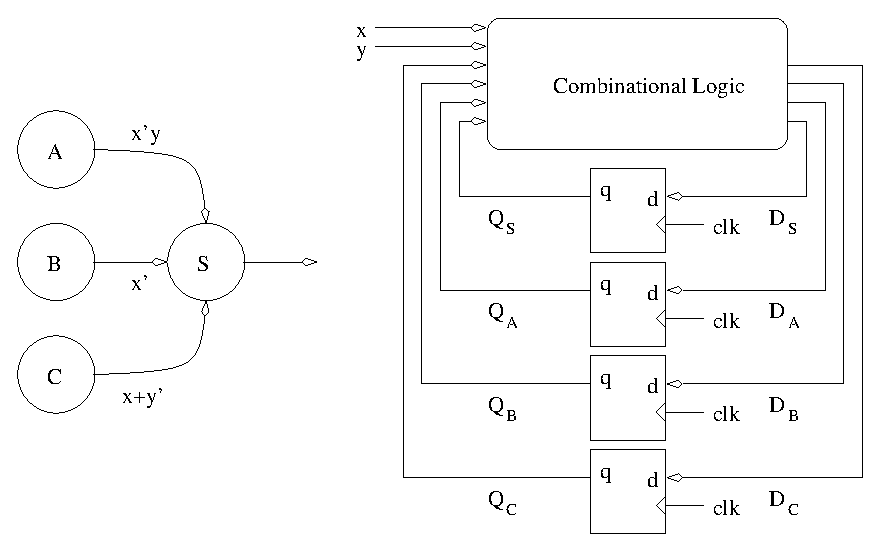
\includegraphics{Ones}}}
    \caption{A state diagram and its FSM.}
    \label{fig:sequentialFSMones}
\end{figure}

The third step in the transformation of a state diagram into a circuit
diagram requires the elaboration of the output bits and the definition of their
value for each state forming an output table.  From Figure~\ref{fig:sequentialFSMGenFSM},
see that the OEs are dependent only on the state.  Remember the
output from the flip flop associated with $S$, $Q_S$, equals 1 when the
FSM is in state $S$.  Consequently, if an output $Z$ equals 1 when the
FSM is in state $S$, then the output equation for $Z$ will contain the
term $Q_S$.  Consulting the output table for a FSM reveals a list
of states for which an output $Z$ equals 1.  Since the output equals
1 when the FSM is in any of these states, the output equation for $Z$
is the logical OR of these states.

The furnace controller circuit first introduced in Chapter 5 is
revisited to better understand the concepts illustrated in
Figure~\ref{fig:sequentialFSMones}.

%%----------------FURNACE CONTROLLER------------

\paragraph{Word Statement}
Design a FSM which controls a furnace in order to regulate the
temperature in a house.  The FSM has two bits of input from thermometer,
$T_{hi}$ and $T_{low}$.  When the temperature inside the house
is greater than the high threshold, then $T_{hi}$ outputs 1; otherwise
it outputs 0.  When the temperature inside the house is greater than
the low threshold, then $T_{low}$ outputs 1; otherwise it outputs 0.
The output from the FSM controls a furnace.  When the FSM outputs a
1, the furnace turns on, warming the house.  When the FSM outputs a 0,
the furnace is turned off, causing the house to cool down.  A graph
of this controller's behavior is given in Figure~\ref{fig:sequentialFSMHysteresisGraph}.

\paragraph{State Diagram}
The FSM has two bits of input and one bit of
output. The state diagram, shown in Figure~\ref{fig:sequentialFSMFurnaceSD}, has
an asterisk in the state \textbf{ OFF} implying that this state is the reset state.
Hence, for start-up, the furnace controller is set in the \textbf{ OFF}
state.

\begin{figure}[ht]
    \center{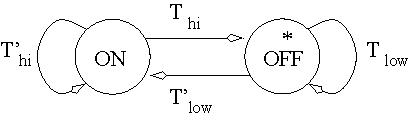
\includegraphics{FurnaceSD}}
    \caption{A state diagram describing the furnace controller.}
    \label{fig:sequentialFSMFurnaceSD}
\end{figure}

\paragraph{Circuit Diagram}
The circuit for the FSM shown in Figure~\ref{fig:sequentialFSMFurnaceSD} requires
two flip flops because it has two states.  These flip flops can be called
ON and OFF, their inputs $D_{on}$ and $D_{off}$, and their outputs
$Q_{on}$ and $Q_{off}$.

The MIEs are derived directly from the state diagram.  Two arcs
terminate at the \textbf{ ON} state, thus the MIE for this state  has
two terms, $D_{on} = Q_{off}*T_{low}' + Q_{on}*T_{hi}'$.  Likewise, the
MIE for the \textbf{ OFF} state has two terms,
$D_{off} = Q_{on}*T_{hi} + Q_{off}*T_{low}$.

In order to determine the OEs, an output table is constructed.  The
table is organized by listing each output as a column and each state as a row.
In the case of the furnace controller, this construction is quite simple.
\\ \\
\begin{tabular}{c||c}

    State        & Furnace    \\ \hline
    & 0 off        \\ \hline
    & 1 on        \\ \hline \hline
    ON        & 1        \\ \hline
    OFF        & 0        \\

\end{tabular}
\\ \\
Since the single output equals 1 when the FSM is in the \textbf{ ON} state,
$Z_{furnace} = Q_{on}$.
Putting all this together yields the complete circuit diagram for the furnace
controller FSM as shown in Figure~\ref{fig:sequentialFSMFurnaceCircuit}.

\begin{figure}[ht]

    \center{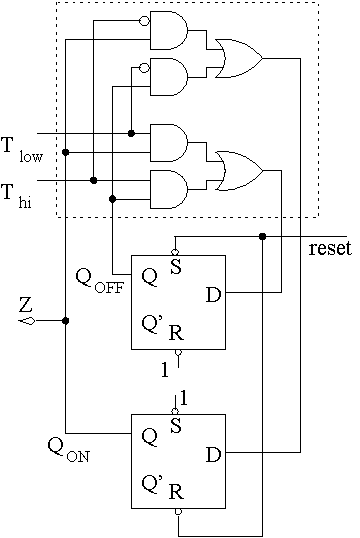
\includegraphics{FurnaceCir}}
    \caption{The circuit diagram for the furnace controller.}
    \label{fig:sequentialFSMFurnaceCircuit}

\end{figure}

One final note needs to be made about the circuit diagram in
Figure~\ref{fig:sequentialFSMFurnaceCircuit}; its reset configuration.  According
to the state diagram shown in Figure~\ref{fig:sequentialFSMFurnaceSD}, the
\textbf{ OFF} state is the reset state.  Hence, the reset signal
is wired to the asynchronous active low set input of the
OFF D flip flop so that its output goes to logic 1 when the
reset is activated.  All the other flip flops are
connected to the reset signal through their asynchronous
active low reset input so that their outputs all go to logic
0 on a reset event.

Since the furnace controller operates through time on real
inputs its behavior is better understood in light of applying
inputs and examining the outputs in a timing diagram.

%%----------------TIMING------------
\section{Timing}
Once the FSM is realized, the only way to inspect the behavior of a physical
realization is by applying inputs and observing outputs.  A timing
diagram is used to examine a sequence of inputs and the resulting behavior of the FSM.
The timing diagram is compared to the state diagram of the FSM in order
to verify that it is operating as originally designed.  Before diving into an
example timing diagram,  the sequence of events
occurring  inside the FSM needs to be understood.

The events occurring in the FSM are referenced to the clock input of the
D flip flops inside the FSM; see Figure~\ref{fig:sequentialFSMGenTime}.  Since flip
flops sample their inputs on the positive edge of the clock, this point is the
beginning of the timing analysis, denoted as Event 1 in
Figure~\ref{fig:sequentialFSMGenTime}.  The propagation delay of the flip flops means
a small delay occurs between the clock edge and the flip flop outputs, $Q$,
becoming valid, Event 2 in Figure~\ref{fig:sequentialFSMGenTime}.  The propagation delay
of the flip flops is denoted $T_{FF}$.  In order to maximize the clocking
frequency of the FSM, the new inputs, $X$, to the FSM should be applied at the
same moment that the flip flop outputs are becoming valid.  This event is Event 3
in Figure~\ref{fig:sequentialFSMGenTime}. According to Figure~\ref{fig:sequentialFSMGenFSM}, changing
$Q$ and $X$ has two effects, the outputs $Z$ change and the memory
inputs $Y$ change.  The delay between the application of the new inputs to
the MIE logic and $Y$ is the propagation delay of the combination logic, denoted
$T_{combo}$ in Figure~\ref{fig:sequentialFSMGenTime}.  Event 4 denotes the instant in time
when $Y$ becomes valid.  When the $Y$ values are valid, a small
delay occurs while the flip flops register their new inputs, denoted $T_{su}$.  After
this setup time, the FSM is ready for another clock edge.

\begin{figure}[ht]

    \center{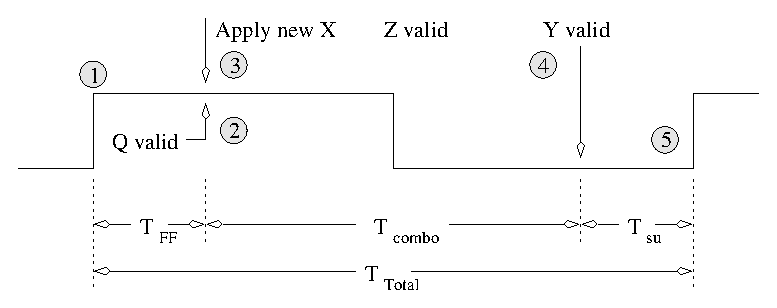
\includegraphics{GenTime}}
    \caption{A timing diagram showing the sequence of events in a FSM.
    The circled numbers refer to the sequence of events in a FSM.}
    \label{fig:sequentialFSMGenTime}

\end{figure}
\label{page:GenTime}
\index{timing!FSM}

The total time between the clock rising and the FSM being ready for another
clock edge, $T_{total} = T_{FF} + T_{combo} + T_{su}$,  is the minimal
amount of time between successive clock edges.  If a clock edge arrived
sooner than $T_{total}$, then at the very least, the setup time of the
flip flops would be violated.  The maximum clocking frequency
of a FSM is $F_{max} = 1/T_{total}$.

Consider the operation of the furnace controller through time.
To do this, consult the memory input equations of the
FSM in Figure~\ref{fig:sequentialFSMFurnaceCircuit}.  A timing diagram, Figure~\ref{fig:sequentialFSMFurnaceTime},
shows a sequence of inputs applied and the
behavior of the circuit. At some time before time=0, the reset signal is
asserted to logic 0.  This reset event causes the FSM to go into the
\textbf{ OFF} state.  The
reset signal is released prior to time=0, but the FSM stays in the \textbf{ OFF}
state because it has not seen a positive clock edge.  At time=0, a positive
clock edge arrives  while the
temperature is below the low threshold. Hence, the furnace transitions
into the \textbf{ ON} state.  The furnace starts producing heat, so the
temperature in the house increases. At
time=15 the temperature goes above the lower threshold, causing
$T_{low}=1$, but the temperature is still below the higher threshold, so $T_{hi}=0$.
The $Q_{on}*T_{hi}'$ term in $D_{on}$ will equal 1, causing the FSM
to transition into the \textbf{ ON} state, during the next clock edge at time=20;
not much of a transition really.  Since the furnace remains on, it is
still producing heat and increasing the temperature in the house.
At time=25, the high temperature threshold is exceeded causing
$T_{hi}=1$ as well as $T_{low}=1$.  The $Q_{on}*T_{hi}$ term of
$D_{off}$ will equal 1, causing the FSM to transition into the \textbf{ OFF}
state at the next positive clock edge at time=30.  With the furnace
off, the temperature in the house starts to drop.  At time=35, the
temperature drops below the high threshold causing $T_{high}=0$,
but still remains above the low threshold causing $T_{low}=1$.
The $Q_{off}*T_{low}$ term of $D_{off}$ equals 1 causing the
FSM to transition into the \textbf{ OFF} state at the next clock edge at
time=40.  Again, this change is not much of a transition because the FSM stays
in the same state.  At time=45, the temperature drops below the low
threshold.  This change causes the $Q_{off}*T_{low}'$ term of $D_{on}$ to
equal 1, causing the FSM to transition to the \textbf{ ON} state at the next
clock edge at time=50.

\begin{figure}[ht]

    \center{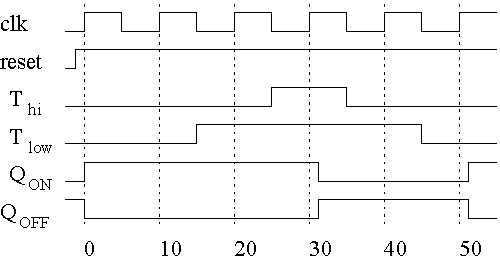
\includegraphics{FurnaceTime}}
    \caption{A timing diagram for the furnace controller.}
    \label{fig:sequentialFSMFurnaceTime}

\end{figure}

The furnace controller is an example of a FSM whose states capture
the operating modes of a system.  The next example, the vending
machine, is a FSM whose states capture the history of the applied
inputs.

%%----------------VENDING MACHINE------------

\section{Vending Machine}
Consider the design of a FSM controlling the operation of a
very basic vending machine.  This machine is not a very user-friendly design
as it does not give out change.

\paragraph{Word Statement}
Design a FSM which has two inputs $N, D$ representing a nickel and a dime,
respectively.  $N=1$ when a nickel has been deposited and $D=1$
when a dime has been deposited. $N$ and $D$ never simultaneously are
equal to 1 because a nickel and a dime cannot be simultaneously
inserted into the coin slot.  The FSM has one output; it equals 1
when 35\textcent~or more has been deposited.  After dispensing a
soda, the FSM should start collecting money for another soda.

\paragraph{State Diagram}
Usually two natural choices can be phrased for what the
FSM is to remember.
\begin{enumerate}
    \item The number of nickels and dimes deposited.
    \item The total amount of money deposited so far.
\end{enumerate}

Clearly, the second approach is going to yield a FSM with far fewer
states, fewer flip flops, and in all likelihood, less logic for the
MIEs.  Hence, use the second approach and move on to
defining the states.  The FSM has eight states:
0\textcent, 5\textcent, $\ldots$ 35\textcent~each representing the total
amount of money deposited so far.  Clearly, 0\textcent~should be the
reset state.  The complete FSM is shown in Figure~\ref{fig:sequentialFSMvend}.

\begin{figure}[ht]

    \center{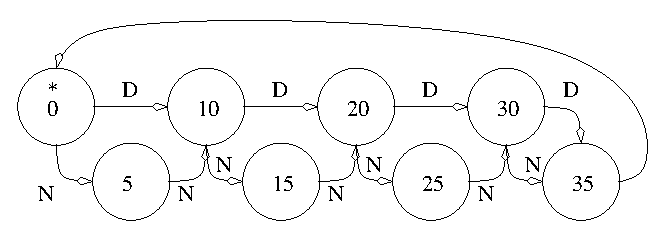
\includegraphics{VendSD}}
    \caption{The state diagram for the vending machine.}
    \label{fig:sequentialFSMvend}

\end{figure}

The state diagram is not complete in the sense of the
definition given on page~\pageref{page:completeness} because it does not
answer the question, ``What happen when no money is deposited?"
It should be obvious that from any state $S$, the transition
arcs labeled $N'$ or $D'$ point back to $S$.  In other words,
if no money is deposited, then the total amount of money
deposited does not change.  These arcs are omitted from the diagram for the
sake of clarity.

Another interesting feature of the state diagram is the arc
leaving state 35\textcent.  The arc is not labeled because
this arc represents an unconditional state transition; the condition on
the arc is assumed to be true regardless of the input
condition.  The FSM spends only one clock cycle in this
state, dispensing a single soda, before transitioning back to state
0\textcent.

Finally, the FSM is not very user-friendly.  A user who deposits
10\textcent~after depositing 30\textcent~gets a soda, but
no change.  The improvement of the FSM is left for a homework
problem.

\paragraph{Circuit Diagram}
The design process of a FSM consists of three steps, determining the
number of flip flops, determining the MIEs, and determining the OEs.
Since the FSM has eight states, the FSM will have eight flip flops,
labeled 0\textcent, 5\textcent, $\ldots$ 35\textcent.

In writing the MIEs, remember every state \textbf{ S} that has an outgoing
arc labeled $N$, also has an undrawn arc labeled $N'$.  This undrawn
arc leaves state \textbf{ S} and returns to state \textbf{ S}.  That is, if a nickel
is not deposited, then the FSM stays in the same state.  Likewise
every state which has an outgoing arc labeled $D$, has an undrawn self arc
labeled $D'$.  For example, three arcs terminate at state 5\textcent.
They are the arc from state 0\textcent labeled $N$ and the two arcs
leaving from state 5\textcent~labeled $N'$ and $D'$.  Hence the MIE
for state 5\textcent~is
$D_{5} = Q_{0}N + Q_{5}N' + Q_{5}D'$ which
can be simplified to
$D_{5} = Q_{0}N + Q_{5}(N' + D')$.  The complete
list of MIEs is given below.

\begin{tabular}{l}

    $D_{35} = Q_{25}D + Q_{30}N + Q_{30}D$ \\
    $D_{30} = Q_{20}D + Q_{25}N + Q_{30}(N'+D')$ \\
    $D_{25} = Q_{15}D + Q_{20}N + Q_{25}(N'+D')$ \\
    $D_{20} = Q_{10}D + Q_{15}N + Q_{20}(N'+D')$ \\
    $D_{15} = Q_{5}D +  Q_{10}N + Q_{15}(N'+D')$ \\
    $D_{10} = Q_{0}D +  Q_{5}N  + Q_{10}(N'+D')$ \\
    $D_{5}  =           Q_{0}N  + Q_{5}(N'+D')$ \\
    $D_{0}  = Q{35} + Q_{0}(N'+D')$ \\

\end{tabular}

A table listing all the states and their output values could be built,
but an inspection of the word statement reveals that the FSM only
outputs 1 when 35\textcent~has been deposited.  Hence, the FSM should
output 1 when it is in state 35\textcent.  Consequently, $Z=Q_{35}$.

%%----------------Wait States------------

\section{Waits States}
When a FSM needs to interface with an entity operating much
slower than the FSM or with an event taking an unknown amount
of time to happen, it is often necessary to include wait states in
the FSM.  A wait state is exactly what its name implies, a state in
which the FSM waits for some input event to occur.

For example, imagine  constructing a FSM to control
a vending machine dispenser.  The FSM asserts its dispense output,
enabling the vending machine to dispense a bag of chips, until its
photodetector detects a bag of chips passing down the
dispense chute.  The photodetector input to the FSM is called
$photo$ and the dispense signal is an output from the FSM.

This FSM has a (wait) state with a self loop labeled
$photo'$ in which it asserts the dispense output.  The FSM is
waiting for the $photo$ input to go to 1, signaling the bag of
chips is being dispensed.  While the \verb+photo+ signal is equal to
0, the FSM asserts the dispense output.  The wait state should have
a second transition arc labeled \verb+photo+ which takes the FSM out
of the wait state when $photo$ equals 1.

The next section illustrates how to incorporate wait states into
a FSM so that it waits patiently for cows to make their way through a
cattle chute.

%%----------------DAISY------------
\section{DAISY}
Consider the design of a FSM capturing the current step of a
process. The task is to design a high-tech cow-tracking system
for a local dairy. The system is called the Dairy Automated Information
SYstem, or DAISY for short.  The system operates as follows.

\paragraph{Word Statement}
Cows have a RFID tag attached to their collars.  When the cow passes through the
cattle chute on their way into the barn, a RFID reader reads the unique
ID stored on the RFID tag and logs the cow into the barn.  The RFID
system outputs a single bit: a 1 means the system has read an
RFID tag and has successfully checked a cow back into the barn; a 0 means
the RFID system is either still processing a tag or is not
currently reading a tag.

In order to ensure each cow is scanned, the flow of cows
into the barn is controlled by two gates at either end of the chute.  Each
gate is controlled by a single bit. To lift a gate, this input must be
held at logic 1; to lower a gate, the input must be held at a logic 0.
The sequence of raising and lowering the gates in order to control the
flow of cows is illustrated in Figure~\ref{fig:sequentialFSMdaisy}.

\begin{figure}[ht]
    \center{\scalebox{0.5}{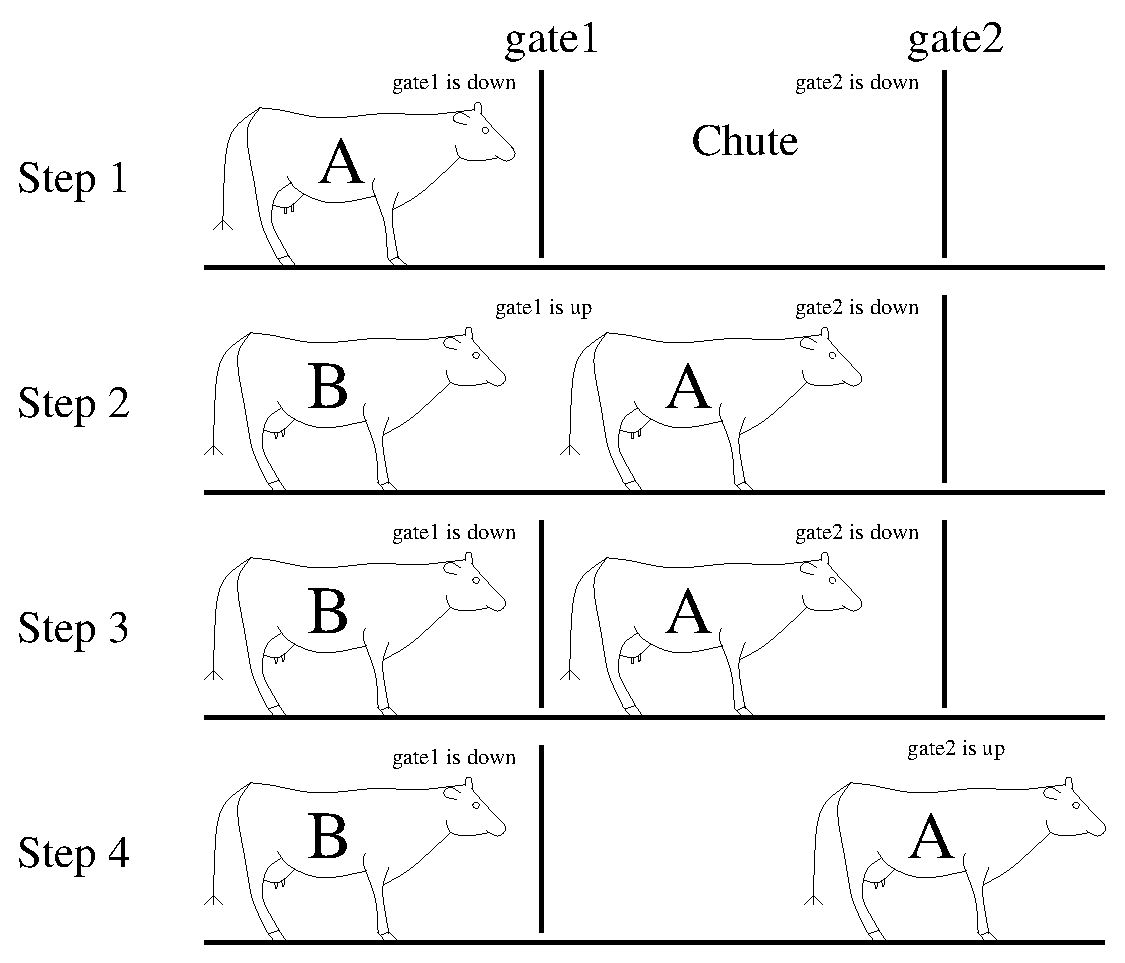
\includegraphics{Daisy}}}
    \caption{The sequence of steps to gate a cow through the RFID reader chute.}
    \label{fig:sequentialFSMdaisy}
\end{figure}

In Step 1, $gate1$ is lifted allowing cow $A$ to enter the chute.
In Step 2, the DAISY system has detected cow $A$ is in the chute and
closes $gate1$.  The cow waits in the closed off chute until the RFID
reader signals that it has read the tag and checked in cow $A$.  The DAISY system
then raises $gate2$ and waits for cow $A$ to leave the chute before closing $gate2$
and transitioning back to Step 1.  If the cow takes more than 30 seconds
to leave the chute, then the cow is ``goosed" by a three-second burst of compressed air.
The compressed air is released by an electronically-controlled valve;
asserting a 1 on the valve's input holds the value open, asserting a
0 closes the air valve.
The system then waits another 30 seconds before firing the air
valve again.  This process continues until the cow leaves the chute.
At any time when the cow leaves the chute, the cycle is
interrupted and the DAISY system transitions back to Step 1.

In order to give DAISY an accurate sense of time, the system is
provided with a single timer with two bits of input and one bit of
output.  To use this timer, set the timer to either 3 or
30 seconds.  By asserting a set command for a single
clock cycle, the timer is set.  Then, the control input commanding the timer to count
down is continuously applied.  The output of the timer will equal
0 until the set time limit has expired at which times its output
will stay at 1 until a new time interval is set.

Before deriving the state diagram, the inputs and outputs of
the DAISY system are categorized.

\paragraph{System Inputs and Outputs}
The word statement infers the existence of three inputs.  The RFID
scanner sends the DAISY system a single bit which indicates if the cow has been
processed.  A second input tells the DAISY system if a cow is in
the chute. The final system input comes from a timer used
to inform the DAISY system when 3 or 30 seconds have expired.
\\ \\
\begin{tabular}{c|c|c}
    RFID Scanner = $r$    & Cow Present = $c$    & Timer Status = $t$    \\ \hline \hline
    1 - Cow checked in    & 1 - cow present    & 1 - timer up        \\ \hline
    0 - Cow not processed    & 0 - no cow        & 0 - timer running    \\
\end{tabular}
\\ \\
The word statement infers the existence of four, separate outputs.  The gates in the
DAISY system are controlled by a single bit each.  Assume
a logic 1 must be continuously applied to a gate in order to keep it raised. In order
to use the timer, set it to either 3 or 30 seconds by applying 01 or
10 for a single clock cycle.  Then, the timer is run by applying 11.  The timer
outputs a status signal (a DAISY input) which should be monitored to tell
DAISY when the set time limit has expired.  When the electronic valve
controlling the compressed air is open, air rushes out, goosing the cow.
\\ \\
\begin{tabular}{c|c|c|c}
    Gate1        & Gate2        & Timer Control            & Air Valve    \\ \hline \hline
    1 - gate up     & 1 - gate up    & 00 Stop timer            & 0 closed    \\ \hline
    0 - gate down    & 0 - gate down    & 01 Set timer to 30 seconds    & 1 open    \\ \hline
    &        & 10 Set timer to 3 seconds    &        \\ \hline
    &        & 11 Run timer            &        \\
\end{tabular}

\paragraph{State Diagram}
The process of creating the state diagram for the DAISY system
requires considering movement through the steps of the process required
to get a single cow through the gated chute.  Each step in this
process then becomes a state or a set of states.  Each state
asserts some output to control the devices connected to
the DAISY system.  Below is one possible list; other arrangements are possible.

\begin{enumerate}
    \item Open gate1
    \item Wait for cow to enter chute
    \item Close gate1
    \item Wait for RFID to read cow
    \item Open gate2
    \item Wait for cow to leave
    \item If 30 seconds has transpired, then ``goose" cow; goto Step 6
    \item Else if the cow has left, then close gate2; goto Step 1
\end{enumerate}

In order to simplify the labels on the state diagram arcs, the inputs
are abbreviated. The RFID scanner input is represented by the variable $r$,
the cow present input is represented by the variable $c$, and the timer
status input is represented by the variable $t$.

\begin{figure}[ht]

    \center{\scalebox{0.7}{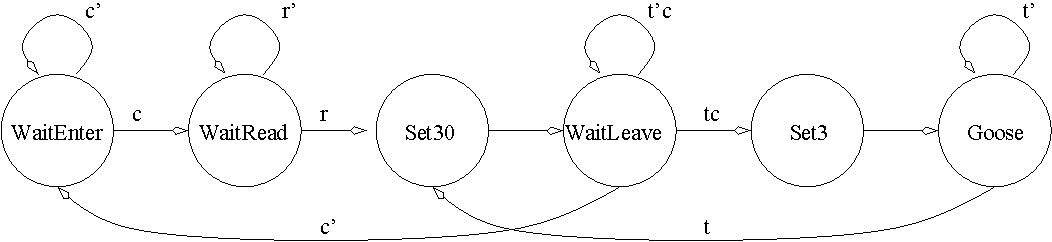
\includegraphics{DaisySD}}}
    \caption{The state diagram for the DAISY system.}
    \label{fig:sequentialFSMdaisySD}

\end{figure}

In some cases the FSM combines a couple of the items
in the list together into a single state.  For example,
Item 1 and Item 2 on the list, ``open gate1" and ``wait for cow
to enter chute" are performed in the \textbf{ WaitEnter} state.  The
``Open gate1" action is performed by asserting the $gate1$
output while in this state.  The ``Wait for cow" action is
performed by the self arc labeled $c'$.  That is, while $c'$ is
true (while $c=0$), the FSM waits in the \textbf{ WaitEnter} state.
After a cow moves into the chute, the system moves into state
\textbf{ WaitRead}.  This state handles Item 3 and Item 4 in the list,
``Close gate1" and ``Wait for RFID to read cow".  Closing the gate
is handled by asserting 0 on the $gate1$ output, while
waiting for the RFID reader is handled by the self arc labeled
$r'$.  When the RFID reader has checked in the cow, the
FSM transitions to the state \textbf{  Set30} where a 30-second count-down is
set.  The FSM then waits for the timer to time-out or for
the cow to leave.

The combinations of timer status and cow present while in the
state \textbf{ WaitLeave} deserves some attention. The state has four
combinations of these two inputs which effect the next state.
In order to reason out the consequences of each input
combination, structuring the analysis can be achieved by putting all
four combinations of inputs into a truth
table.  Then, each combination can be carefully analyzed to
determine which next state occurs as well as to simplify the
expressions placed on the arcs.

\begin{table}
    \begin{tabular}{c|c||c|c}
        Timer Status     & Cow Present     & Action        & Next State    \\ \hline \hline
        0            & 0            & close gate2    & WaitEnter        \\ \hline
        0            & 1            & wait        & WaitLeave        \\ \hline
        1            & 0            & close gate2    & WaitEnter        \\ \hline
        1            & 1            & goose the cow    & Set3, Goose        \\
    \end{tabular}
\end{table}

The pair of transitions which lead to the \textbf{ WaitEnter} state can be
simplified by noting that in both cases, the cow present status
bit is 0 (denoted by $c'$ on the state diagram).

\paragraph{Memory Input Equations}
Since the FSM is built with a one-hot encoding of the states,
then the MIEs are formed by answering the question, ``How did
I get into this state?"  The answer to this question, answered
for each state is given below.

\begin{tabular}{l}
    $D_{WaitEnter}    = Q_{WaitEnter}c' + Q_{WaitLeave}c'$  \\
    $D_{WaitRead}    = Q_{WaitEnter}c + Q_{WaitRead}r'$ \\
    $D_{Set30}    = Q_{WaitRead}r + Q_{Goose}t$ \\
    $D_{WaitLeave}    = Q_{Set30} + Q_{WaitLeave}t'c$ \\
    $D_{Set3}    = Q_{WaitLeave}tc$ \\
    $D_{Goose}    = Q_{Set3} +  Q_{Goose}t'$ \\
\end{tabular}

\paragraph{Output Equations}
The output table is shown in Table~\ref{table:daisy}.  The table is
referred to as the \textit{ control word} table.  The term
``control" is used because the table describes how the FSM controls
its associated hardware.  The term ``word" is used to indicate
the control is formed from a collection of bits.

\begin{table}[ht]
    {\small
        \begin{tabular}{c||c|c|c|c}
            State        & Gate1        & Gate2        & Timer Control            & Air        \\ \hline \hline
            & 1 - gate up    & 1 - gate up    & 00 Stop timer            & 0 - closed \\ \hline
            & 0 - gate down    & 0 - gate down    & 01 Set timer to 30 seconds    & 1 - open    \\ \hline
            &            &            & 10 Set timer to 3 seconds    &        \\ \hline
            &            &            & 11 Run timer            &         \\ \hline \hline
            \textbf{ WaitEnter}    & 1            & 0            & 00                    & 0        \\ \hline
            \textbf{ WaitRead}    & 0            & 0            & 00                    & 0        \\ \hline
            \textbf{ Set30}        & 0            & 0            & 01                    & 0        \\ \hline
            \textbf{ WaitLeave}    & 0            & 1            & 00                    & 0        \\ \hline
            \textbf{ Set3}        & 0            & 0            & 10                    & 0        \\ \hline
            \textbf{ Goose}        & 0            & 0            & 11                    & 1        \\
        \end{tabular}
    }
    \label{table:daisy}
\end{table}

The output equations are derived by looking at the columns
of the control word table.  Each column is given its own
output equation by asking, ``What states cause this
output to go to 1?"  ORing together these states produced
the output equation for the corresponding output.  For
example, the $Gate1$ output only goes to logic 1 when the
FSM is in the \textbf{ WaitEnter} state, hence
$Z_{Gate1} = Q_{WaitEnter}$.  The complete list of output
equations is given below.

\begin{tabular}{l}

    $Z_{Gate1}    = Q_{WaitEnter}$  \\
    $Z_{Gate2}    = Q_{WaitLeave}$ \\
    $Z_{Timer1}    = Q_{Set3} + Q_{Goose}$ \\
    $Z_{Timer0}    = Q_{Set30} + Q_{Goose}$ \\
    $Z_{Air}    = Q_{Goose}$ \\
\end{tabular}
